\documentclass[conference]{IEEEtran}
\IEEEoverridecommandlockouts
% The preceding line is only needed to identify funding in the first footnote. If that is unneeded, please comment it out.
%Template version as of 6/27/2024

\usepackage{cite}
\usepackage{amsmath,amssymb,amsfonts}
\usepackage{algorithm}
\usepackage{algpseudocode}
\usepackage{booktabs}
\usepackage{flushend}
\usepackage{graphicx}
\usepackage{tikz}
\usepackage{textcomp}
\usepackage{xcolor}
\usetikzlibrary{arrows,positioning,shapes.geometric}
\def\BibTeX{{\rm B\kern-.05em{\sc i\kern-.025em b}\kern-.08em
    T\kern-.1667em\lower.7ex\hbox{E}\kern-.125emX}}
\begin{document}

\title{Conference Paper Title*\\
{\footnotesize \textsuperscript{*}Note: Sub-titles are not captured for https://ieeexplore.ieee.org  and
should not be used}
\thanks{Identify applicable funding agency here. If none, delete this.}
}

\author{\IEEEauthorblockN{1\textsuperscript{st} Given Name Surname}
\IEEEauthorblockA{\textit{dept. name of organization (of Aff.)} \\
\textit{name of organization (of Aff.)}\\
City, Country \\
email address or ORCID}
\and
\IEEEauthorblockN{2\textsuperscript{nd} Given Name Surname}
\IEEEauthorblockA{\textit{dept. name of organization (of Aff.)} \\
\textit{name of organization (of Aff.)}\\
City, Country \\
email address or ORCID}
\and
\IEEEauthorblockN{3\textsuperscript{rd} Given Name Surname}
\IEEEauthorblockA{\textit{dept. name of organization (of Aff.)} \\
\textit{name of organization (of Aff.)}\\
City, Country \\
email address or ORCID}
\and
\IEEEauthorblockN{4\textsuperscript{th} Given Name Surname}
\IEEEauthorblockA{\textit{dept. name of organization (of Aff.)} \\
\textit{name of organization (of Aff.)}\\
City, Country \\
email address or ORCID}
\and
\IEEEauthorblockN{5\textsuperscript{th} Given Name Surname}
\IEEEauthorblockA{\textit{dept. name of organization (of Aff.)} \\
\textit{name of organization (of Aff.)}\\
City, Country \\
email address or ORCID}
\and
\IEEEauthorblockN{6\textsuperscript{th} Given Name Surname}
\IEEEauthorblockA{\textit{dept. name of organization (of Aff.)} \\
\textit{name of organization (of Aff.)}\\
City, Country \\
email address or ORCID}
}

\maketitle

\begin{abstract}
This document is a model and instructions for \LaTeX.
This and the IEEEtran.cls file define the components of your paper [title, text, heads, etc.]. *CRITICAL: Do Not Use Symbols, Special Characters, Footnotes, 
or Math in Paper Title or Abstract.
\end{abstract}

\begin{IEEEkeywords}
component, formatting, style, styling, insert.
\end{IEEEkeywords}

\section{Introduction}
\subsection{Background and Motivation}
IoT networks now connect household appliances, industrial controllers, and public-service devices that generate markedly different traffic patterns. A compromised endpoint can provide a route to other devices or services. Identifying malicious traffic is therefore only part of the problem. A useful network intrusion detection system (NIDS) must distinguish attack categories, not merely separate benign from malicious flows. CIC-ToN-IoT provides labeled IoT network flows for this multiclass setting, although its heterogeneous features and sharply unequal class frequencies remain challenging for machine-learning models \cite{Sarhan2022,Ma2025FSLLM}.

\subsection{Challenges}
High dimensionality and class imbalance create related modeling problems. Some traffic features are redundant or carry little signal, adding complexity without improving class separation. Meanwhile, majority classes can dominate training; high accuracy may coexist with poor detection of rare attacks. Accuracy alone hides this. Preprocessing introduces a separate risk. If normalization or other data-dependent steps are applied before splitting, information from held-out flows can enter training and make test results look stronger than they are \cite{Bouke2023,Manocchio2025}. An Autoencoder can learn a compact, nonlinear representation \cite{Zhang2023SIGMOD,Li2024FeatureReduction}, while Light Gradient Boosting Machine (LightGBM) is well suited to tabular intrusion data \cite{Liu2021LightGBM,Munawar2025,Wakili2025}.

\subsection{Approach and Contributions}
Our pipeline begins with all 5,351,760 raw CIC-ToN-IoT flow records. After invalid rows and non-informative fields are removed, 69 traffic features remain. We use a stratified 80:20 train--test split and fit MinMax scaling only on the training partition. The Autoencoder maps the 69 features to a 16-dimensional latent representation, which LightGBM classifies under four training-data treatments: no imbalance handling, class weighting, random upsampling, and random downsampling. Every scenario uses the original, untouched test distribution. We also train LightGBM directly on the 69 normalized features to measure how much discriminative information the latent representation retains.

We make three contributions. First, we implement an end-to-end multiclass NIDS pipeline on the full dataset with explicit controls against preprocessing and test-set leakage. Second, we compare four imbalance-handling scenarios using accuracy, macro precision, macro recall, macro F1-score, per-class metrics, and confusion matrices, which exposes their effects on minority attacks. Third, we contrast the 16-feature latent representation with the original 69-feature representation, quantifying the trade-off between dimensionality reduction and discriminative performance rather than assuming that compression necessarily improves classification.

\section{Related Work}
\subsection{Detection Paradigms}
Intrusion detection can be organized by what is monitored and how attacks are recognized. Host-based systems inspect activity on individual machines, whereas NIDS analyzes traffic flowing between devices. Signature-based detectors match known patterns and work well when attack definitions already exist; anomaly-based detectors instead flag deviations from learned normal behavior and can expose previously unseen attacks, usually at the cost of more false alarms \cite{Rahman2025,Alfahaid2025}. For IoT traffic, centralized network monitoring avoids requiring an agent on every constrained device \cite{Hassan2025IoMT}. Research has also shifted from binary benign--attack decisions toward multiclass labels that identify attack families \cite{Sarhan2022,Ma2025FSLLM}. The added detail is operationally useful, but similar traffic signatures and rare classes make the classification problem harder.

\subsection{Feature Reduction}
Feature reduction addresses the redundancy found in many network attributes. Feature selection retains a subset of the original attributes, preserving their meaning and making model behavior easier to trace \cite{Li2024FSvsFE,Achbarou2026}. Feature extraction instead transforms the inputs into a new representation \cite{Li2024FSvsFE,Li2024FeatureReduction}. Principal Component Analysis provides a linear projection, whereas Autoencoders can capture nonlinear dependencies; sparse and stacked sparse variants further constrain or deepen that representation \cite{Yao2023,Xiao2024,Zhang2023SIGMOD}. Several intrusion-detection pipelines therefore place an encoder before a separate classifier \cite{HariVinayak2025,Ayad2025}. We follow that arrangement but retain an original-feature baseline, since low reconstruction error does not guarantee that the latent space preserves every class boundary.

\subsection{Gradient Boosting and Imbalance Handling}
Boosted tree models remain strong candidates for tabular network data. LightGBM builds an ensemble of decision trees efficiently, and prior NIDS studies have combined it with oversampling, feature selection, or optimization \cite{Liu2021LightGBM,Munawar2025,Wakili2025,Kouassi2025}. These combinations matter because imbalance treatments change what the classifier learns: class weights alter each class's contribution without changing the sample set, upsampling adds minority observations, and downsampling removes majority observations \cite{Ma2025FSLLM,Wakili2025}. The balanced weight assigned to class $c$ is
\begin{equation}
w_c = \frac{n}{C \cdot n_c},
\label{eq:class_weight}
\end{equation}
where $n$ is the number of training samples, $C$ is the number of classes, and $n_c$ is the number of training samples in class $c$. Each choice can trade majority-class performance for minority-class recall. Comparisons on an unchanged test distribution and with macro-averaged metrics are therefore more informative than accuracy alone. Our experiments hold preprocessing, representation, classifier settings, and test data fixed so that differences among the four imbalance scenarios can be attributed to the training-data treatment.

\section{Methodology}
The experimental workflow and model architecture are shown in Figs.~\ref{fig:method_flow} and~\ref{fig:ae_lgbm_architecture}. Dataset inspection precedes every learned transformation, and all parameters are estimated without access to the test partition.

\begin{figure}[t]
\centering
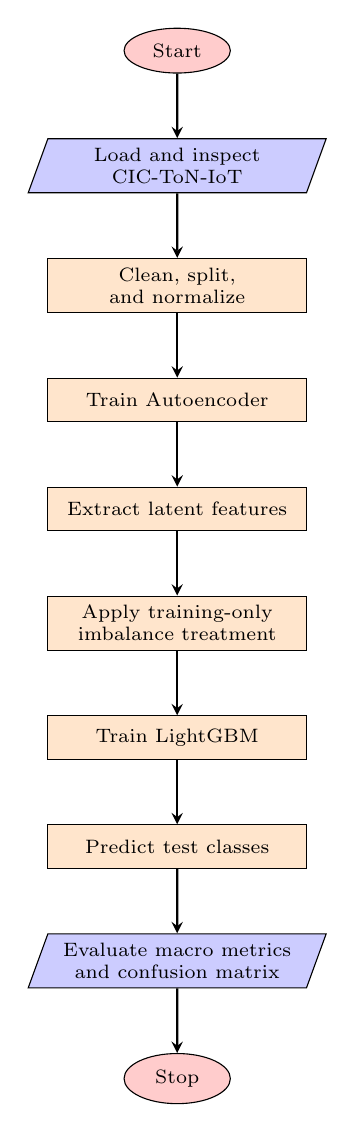
\begin{tikzpicture}[
    node distance=0.82cm,
    startstop/.style={
        ellipse,
        draw=black,
        fill=red!20,
        minimum width=1.35cm,
        minimum height=0.45cm,
        align=center,
        font=\scriptsize
    },
    io/.style={
        trapezium,
        trapezium left angle=70,
        trapezium right angle=110,
        draw=black,
        fill=blue!20,
        text width=3.05cm,
        minimum height=0.55cm,
        align=center,
        font=\scriptsize
    },
    process/.style={
        rectangle,
        draw=black,
        fill=orange!20,
        text width=3.05cm,
        minimum height=0.55cm,
        align=center,
        font=\scriptsize
    },
    flowarrow/.style={thick,->,>=stealth}
]
\node (start) [startstop] {Start};
\node (load) [io, below=of start] {Load and inspect CIC-ToN-IoT};
\node (prep) [process, below=of load] {Clean, split, and normalize};
\node (ae) [process, below=of prep] {Train Autoencoder};
\node (latent) [process, below=of ae] {Extract latent features};
\node (scenario) [process, below=of latent] {Apply training-only imbalance treatment};
\node (lgbm) [process, below=of scenario] {Train LightGBM};
\node (predict) [process, below=of lgbm] {Predict test classes};
\node (evaluate) [io, below=of predict] {Evaluate macro metrics and confusion matrix};
\node (stop) [startstop, below=of evaluate] {Stop};
\draw [flowarrow] (start) -- (load);
\draw [flowarrow] (load) -- (prep);
\draw [flowarrow] (prep) -- (ae);
\draw [flowarrow] (ae) -- (latent);
\draw [flowarrow] (latent) -- (scenario);
\draw [flowarrow] (scenario) -- (lgbm);
\draw [flowarrow] (lgbm) -- (predict);
\draw [flowarrow] (predict) -- (evaluate);
\draw [flowarrow] (evaluate) -- (stop);
\end{tikzpicture}
\caption{Leakage-controlled Autoencoder--LightGBM workflow.}
\label{fig:method_flow}
\end{figure}

\begin{figure*}[t]
\centering
\resizebox{\textwidth}{!}{%
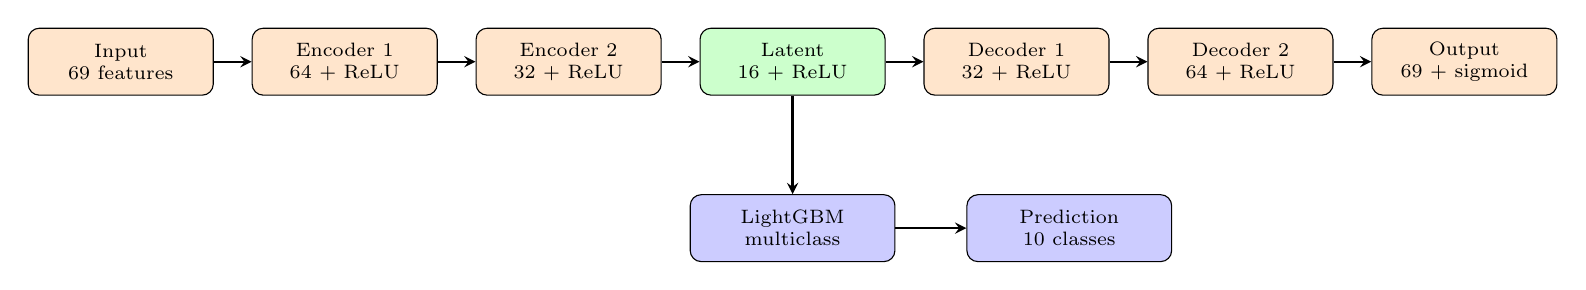
\begin{tikzpicture}[
    node distance=0.48cm,
    layer/.style={
        rectangle,
        rounded corners,
        draw=black,
        fill=orange!20,
        minimum width=2.35cm,
        minimum height=0.85cm,
        align=center,
        font=\scriptsize
    },
    latent/.style={
        rectangle,
        rounded corners,
        draw=black,
        fill=green!20,
        minimum width=2.35cm,
        minimum height=0.85cm,
        align=center,
        font=\scriptsize
    },
    classifier/.style={
        rectangle,
        rounded corners,
        draw=black,
        fill=blue!20,
        minimum width=2.6cm,
        minimum height=0.85cm,
        align=center,
        font=\scriptsize
    },
    modelarrow/.style={thick,->,>=stealth}
]
\node (input) [layer] {Input\\69 features};
\node (enc1) [layer, right=of input] {Encoder 1\\64 + ReLU};
\node (enc2) [layer, right=of enc1] {Encoder 2\\32 + ReLU};
\node (latentnode) [latent, right=of enc2] {Latent\\16 + ReLU};
\node (dec1) [layer, right=of latentnode] {Decoder 1\\32 + ReLU};
\node (dec2) [layer, right=of dec1] {Decoder 2\\64 + ReLU};
\node (output) [layer, right=of dec2] {Output\\69 + sigmoid};
\node (lgbm) [classifier, below=1.25cm of latentnode] {LightGBM\\multiclass};
\node (prediction) [classifier, right=0.9cm of lgbm] {Prediction\\10 classes};
\draw [modelarrow] (input) -- (enc1);
\draw [modelarrow] (enc1) -- (enc2);
\draw [modelarrow] (enc2) -- (latentnode);
\draw [modelarrow] (latentnode) -- (dec1);
\draw [modelarrow] (dec1) -- (dec2);
\draw [modelarrow] (dec2) -- (output);
\draw [modelarrow] (latentnode) -- (lgbm);
\draw [modelarrow] (lgbm) -- (prediction);
\end{tikzpicture}%
}
\caption{Autoencoder--LightGBM architecture. The Autoencoder is optimized with MSE and Adam; only the encoder path supplies features to LightGBM.}
\label{fig:ae_lgbm_architecture}
\end{figure*}

\subsection{Dataset}
The raw CIC-ToN-IoT CSV contains 5,351,760 network-flow records and 85 columns. The \texttt{Attack} field defines one benign and nine attack classes. Table~\ref{tab:dataset_distribution} reports the pre-cleaning distribution and shows the severe skew: Benign and XSS account for 87.16\% of all flows, whereas DDoS and DoS contain only 202 and 145 records, respectively \cite{Sarhan2022,Ma2025FSLLM}.

\begin{table}[t]
\caption{Raw CIC-ToN-IoT Summary and Class Distribution}
\label{tab:dataset_distribution}
\centering
\footnotesize
\setlength{\tabcolsep}{4pt}
\renewcommand{\arraystretch}{0.92}
\begin{tabular}{@{}lrr@{}}
\toprule
\textbf{Class} & \textbf{Records} & \textbf{Share (\%)} \\
\midrule
Benign     & 2,515,236 & 46.998 \\
Backdoor   &    27,145 &  0.507 \\
DDoS       &       202 &  0.004 \\
DoS        &       145 &  0.003 \\
Injection  &   277,696 &  5.189 \\
MITM       &       517 &  0.010 \\
Password   &   340,208 &  6.357 \\
Ransomware &     5,098 &  0.095 \\
Scanning   &    36,205 &  0.677 \\
XSS        & 2,149,308 & 40.161 \\
\midrule
\textbf{Total} & \textbf{5,351,760} & \textbf{100.000} \\
\bottomrule
\end{tabular}
\end{table}

\subsection{Preprocessing}
Identifier and metadata columns, including flow identifiers, endpoint addresses, and timestamps, were excluded together with empirically constant or uninformative fields, leaving 69 numerical features. Removing 1,177 rows with invalid numerical values left 5,350,583 observations. Label encoding was followed by a stratified 80:20 split, producing 4,280,466 training and 1,070,117 test rows. MinMax parameters were fitted only on the training partition and then applied unchanged to both splits. Resampling and class weighting were likewise restricted to training data \cite{Bouke2023,Manocchio2025}.

\subsection{Autoencoder}
The symmetric Autoencoder maps 69 normalized inputs through dense layers of 64 and 32 units to a 16-unit latent layer, then reconstructs them through 32 and 64 units to a 69-unit output. Hidden and latent layers use ReLU; the output uses sigmoid. Training uses mean squared error and Adam for 50 epochs with a batch size of 4096 and a learning rate of 0.001. Mini-batches are reshuffled each epoch, and the checkpoint with the lowest validation loss is retained. Fig.~\ref{fig:ae_lgbm_architecture} shows both reconstruction and classification paths.

\subsection{Latent Extraction and Imbalance Scenarios}
The selected encoder transforms both normalized splits into 16-dimensional arrays, denoted by $Z_{\mathrm{train}}$ and $Z_{\mathrm{test}}$. Only $Z_{\mathrm{train}}$ and $y_{\mathrm{train}}$ are modified by the scenarios in Table~\ref{tab:imbalance_scenarios}; $Z_{\mathrm{test}}$ remains byte-identical throughout. Scenario S2 uses the balanced weights defined in \eqref{eq:class_weight}.

\begin{table}[t]
\caption{Training-Data Imbalance Scenarios}
\label{tab:imbalance_scenarios}
\centering
\footnotesize
\setlength{\tabcolsep}{4pt}
\renewcommand{\arraystretch}{0.95}
\begin{tabular}{@{}cl@{}}
\toprule
\textbf{ID} & \textbf{Training treatment} \\
\midrule
S1 & No imbalance handling \\
S2 & Balanced class weights from \eqref{eq:class_weight} \\
S3 & Random upsampling to the largest class \\
S4 & Random downsampling to 116 samples per class \\
\bottomrule
\end{tabular}
\end{table}

\subsection{LightGBM and Evaluation}
Each scenario trains LightGBM with a multiclass objective, 10 classes, 200 estimators, a learning rate of 0.05, at most 31 leaves per tree, and deterministic seed 42. The fixed estimator count is used without an internal validation split or early stopping. Predictions on the unchanged test set are evaluated using accuracy, macro precision, macro recall, macro F1-score, per-class scores, and a $10\times10$ confusion matrix \cite{Liu2021LightGBM,Wakili2025}.

\subsection{Core Algorithm}
Algorithm~\ref{alg:ae_lgbm_pipeline} summarizes the shared modeling path after preprocessing. The class-weight expression is referenced rather than repeated.

\begin{algorithm}[H]
\footnotesize
\caption{Core Autoencoder--LightGBM Pipeline}
\label{alg:ae_lgbm_pipeline}
\begin{algorithmic}[1]
\Require $X_{\mathrm{train}}^{\mathrm{norm}}$, $X_{\mathrm{test}}^{\mathrm{norm}}$, $y_{\mathrm{train}}$, $y_{\mathrm{test}}$
\Require imbalance scenario $S \in \{S1,S2,S3,S4\}$
\Ensure evaluation result $R$
\State Train Autoencoder $\theta^*$ on $X_{\mathrm{train}}^{\mathrm{norm}}$ by minimizing MSE
\State $Z_{\mathrm{train}} \gets \operatorname{Encoder}_{\theta^*}(X_{\mathrm{train}}^{\mathrm{norm}})$
\State $Z_{\mathrm{test}} \gets \operatorname{Encoder}_{\theta^*}(X_{\mathrm{test}}^{\mathrm{norm}})$
\If{$S=S1$}
    \State Keep $Z_{\mathrm{train}}$ and $y_{\mathrm{train}}$ unchanged
\ElsIf{$S=S2$}
    \State Assign class weights using \eqref{eq:class_weight}
\ElsIf{$S=S3$}
    \State Upsample minority classes in the training set
\ElsIf{$S=S4$}
    \State Downsample majority classes in the training set
\EndIf
\State $M \gets \operatorname{TrainLightGBM}(Z_{\mathrm{train}},y_{\mathrm{train}},S)$
\State $\hat{y}_{\mathrm{test}} \gets M(Z_{\mathrm{test}})$
\State $R \gets \operatorname{Evaluate}(y_{\mathrm{test}},\hat{y}_{\mathrm{test}})$
\State \Return $R$
\end{algorithmic}
\end{algorithm}

\bibliographystyle{IEEEtran}
\bibliography{References}

\end{document}
